\chapter{Literature Survey}\label{ch:literature-survey}
\mycomment{
    Include a bit of text here to explain the structure of this section.

    * remember to do some comparisons between papers! 
    * this section should look at trends in the area of my  research
    * fake-ness (or 'synthetic'-ness) is correct!

    Try and stick some figures in to spice it up a bit, currently reads a tad bare
  }

\section{Automatic Speech Recognition}\label{sec:what-is-asr}

\subsection{What is ASR?}

Automatic Speech Recognition (ASR) is a technology which allows computers to recognise and produce a text transcription of spoken language.
The research and development of technology involving speech has been a part of computer science since the late 1930s\cite{Rabiner2004Jan,vocoder}, with rudimentary ASR systems being constructed as early as the 1950s\cite{asr-52}.
These early attempts at recognising human speech treated it as a `pattern matching' problem, the theory being that words could be constructed by matching the pattern created in a speech signal to corresponding spoken phonemes\cite{Rabiner2004Jan}. 
This paradigm falls apart when the system must be re-tuned for each individual, even for simple tasks such as recognising spoken digits\cite{asr-52}, due to the fact that individual speakers don't produce exactly the same signal for each phoneme\cite{Horton2010}.

Since the 1970s, finding the solution to the problem of pattern matching for speech recognition has been considered unviable through the precise matching of patterns but instead finding the most probable pattern using statistical modelling\cite{Rabiner2004Jan}.
The method which became most widely adopted and is still at the heart of modern ASR is Hidden Markovian Modelling, which was first applied to ASR in the '70s\cite{baker1975stochastic} and continued through the '90s\cite{bengio1999markovian} until today\cite{hmm2023}.

\subsection{Hidden Markov Models}

In his 1960 work\cite{dynkin1960}, Dynkin describes a Markov process using the example of a randomly-moving particle in space;

\say{
        If the position of the particle is known at the instant $t$, supplementary information regarding the phenomena observed up till the instant $t$ (and in particular, regarding the nature of the motion until $t$) has no effect on prognosis of the motion after the instant $t$ (for a known "present", the "future" and the "past" are independent of each other).
}

From his description, we can draw the following assumptions for modelling a system as a Markov process;

\begin{itemize}
  \item The system consists of states.
  \item The system is \emph{in motion}, i.e. moving between states.
  \item This motion is random.
  \item The motion observed prior to $t$ (say, $t-1$) does not influence $t+k$ where $k \geq 1$.
  \item Because the particle is constantly moving between states, the state at time $t$ depends only on the state immediately prior, $t-1$.
  \item There is some probability, $p$, that the system moves from one state to another.
\end{itemize}

In a \emph{Hidden} Markov Model (HMM), the states and transition probabilities between them are known, but for some output sequence the order and selection of states used to produce the output is not known.
Knowing both the states and transition probabilities, it is therefore possible to calculate the most probable set of inputs used to produce the output.

To apply this model to speech, treat speech as a continuous sequence of discrete states, where each state is a feature vector representing an acoustic signal (either whole words, phonemes or even sub-phonetic features\cite{bengio1999markovian}).
Assuming that each state is generated from a probabilistic distribution correlated with other states in the model\cite{Rabiner1989Feb} (i.e. probability that one state follows another) and having trained these distributions on known data, the output signal (i.e. the speech signal) can be used to determine the most probable sequence of tokens spoken.
These tokens may then be decoded by a language model to construct a transcription\cite{bengio1999markovian}.

Despite making up much of the research foundational to modern ASR, Markov models have a crucial flaw when applied to speech; parts of speech are dependent on more than just the part immediately before (i.e. $t-1$).
For instance, in a presentation discussing \emph{hats} it is unlikely that the word \emph{cat} would be used, despite the phonetics of the word being largely the same.

\subsection{How Does Modern ASR Work?}

Skipping ahead from the mid-1980s to the current day, ASR has moved towards what is known as the 'end-to-end' or 'encoder-decoder' model;
at a high level, the input audio is encoded into features, these features are aligned with language and then decoded to produce an output transcript\cite{wang2019overview}.
The key difference between modern approaches and the classical HMM-based approach is the use of widely researched 'machine-learning' techniques, including various forms of neural network\cite{mustafa2019comparative, amodei2016deep, hori2017advances, Kim2017Mar}.

Recent research has proposed a new network architecture called the \emph{Transformer}\cite{vaswani2017attention}, aiming to reduce the computational complexity of encoder-decoder models by forgoing convolutional or recurrent neural networks (CNNs and RNNs) and instead relying on 'self-attention'.
The motivation for the \emph{Transformer} can be understood as follows;

\begin{itemize}
        \item CNNs (e.g. \cite{zeghidour2018fully}) and RNNs (e.g. \cite{graves2014towards}), while popular, have greater per-layer computational complexity than self-attention\cite{vaswani2017attention}.
        \item Recurrent neural networks must perform $O(n)$ sequential operations for a sequence length $n$, whereas self-attention has a constant (i.e. $O(1)$) maximum number of sequential operations, enabling parallel computation\cite{vaswani2017attention}.
        \item By allowing each layer in the encoder and decoder to attend to the whole output of the previous layer, 
\end{itemize}

In a multilayer network, self-attention layers are used to build relations between separate parts of an input sequence by allowing each node (or 'attention head'\cite{shaw2018self}) to attend to all outputs from the previous layer.

\mycomment{ perhaps delete this part? I'd rather not get bogged down in maths...}
According to the work that introduced it\cite{vaswani2017attention}, attention in the Transformer architecture is calculated as;

\[ \text{Attention}(Q,K,V) = \text{softmax}(\frac{QK^T}{\sqrt{d_k}})V \]

Where;

\begin{itemize}
        \item $Q$ is the Query
        \item ...
\end{itemize}


\mycomment{
        Replace 'self-attention' with 'attention' - we're using both self- and cross-attention
        Explain parameters for attention and link to speech recognition.
        Explained in vaswani2017 and shaw2018.
        QKV and O are all weighted - these weights create decision boundaries
        Transformer uses attention in encoding AND decoding
        }

\subsection{Evaluating ASR Systems}
\mycomment{
        Write about WER, PER, CER etc. 
        WER is most used (back this statement up)
        Caveats for using WER
        }

\subsection{Problems in ASR}

Despite their ubiquity, modern ASR systems aren't without fault.
Cutting edge systems like \emph(wav2vec) are touted as being capable of achieving 'greater-than-human' scores on specific datasets\cite{wav2vec2,bigssl,chung2021} such as \emph{LibriSpeech}\cite{librispeech}, achieving as low as 1.4\% error\cite{zhang2020}.

A major problem with comes when the data is not `clean', for example, background noise is present, microphones are far away, the speaker has an atypical speech pattern, etc. 
In this setting, \emph{wav2vec} achieves much poorer scores with word error rates as high as 65\%\cite{whisper} on the \emph{CHiME6} corpus\cite{chime6}.

\mycomment{
        do more on problems here. set the scene for why transcription can't just be performed entirely by a computer (to be expanded on in the section about semi-/full-auto transcription)
    }

\section{Whisper}

In late September 2022, the OpenAI research laboratory (known for such projects as GPT-3/4 and ChatGPT) released a new open-source ASR system known as `Whisper'~\cite{whisper}.
Whisper is unique in being very large (trained on 680,000 hours of speech data), open-source, and fully supervised;
all the training data used to create the model has been accurately labeled and quality-checked by humans, unlike much larger unsupervised (or semi-supervised) models such as `BigSSL' (1,000,000+ hours of data)~\cite{bigssl}.

Unsupervised training is appealing for training speech recognisers because there is a wealth of unlabeled recordings, and labeled recordings are uncommon for less widely-spoken languages\cite{baevski2021}.
Unsupervised systems have a clear disadvantage, however, when compared to supervised; they lack clear decoder mappings\cite{whisper}, meaning that even for a successfully encoded input there may not be a clear mapping from that input into a speech token.
To solve this, fine-tuning to map encodings to decoded text tokens is done on the part of the model's developers, though this is a precarious route to overfitting;
if the model is too fine-tuned to its training data, performance will suffer when faced with data which isn't well represented in the training set.

For example, if an unsupervised model were trained using the voices of young people, it may perform with considerably poorer accuracy when used to transcribe elderly speakers due to differences inherent to their speech\cite{Horton2010}.

\subsection{Operation}

Whisper is an encoder-decoder transformer, though it uses 'learned positional encodings' to \mycomment{ EXPLAIN HOW WHISPER WORKS HERE!!! }

\begin{figure}[h!]
  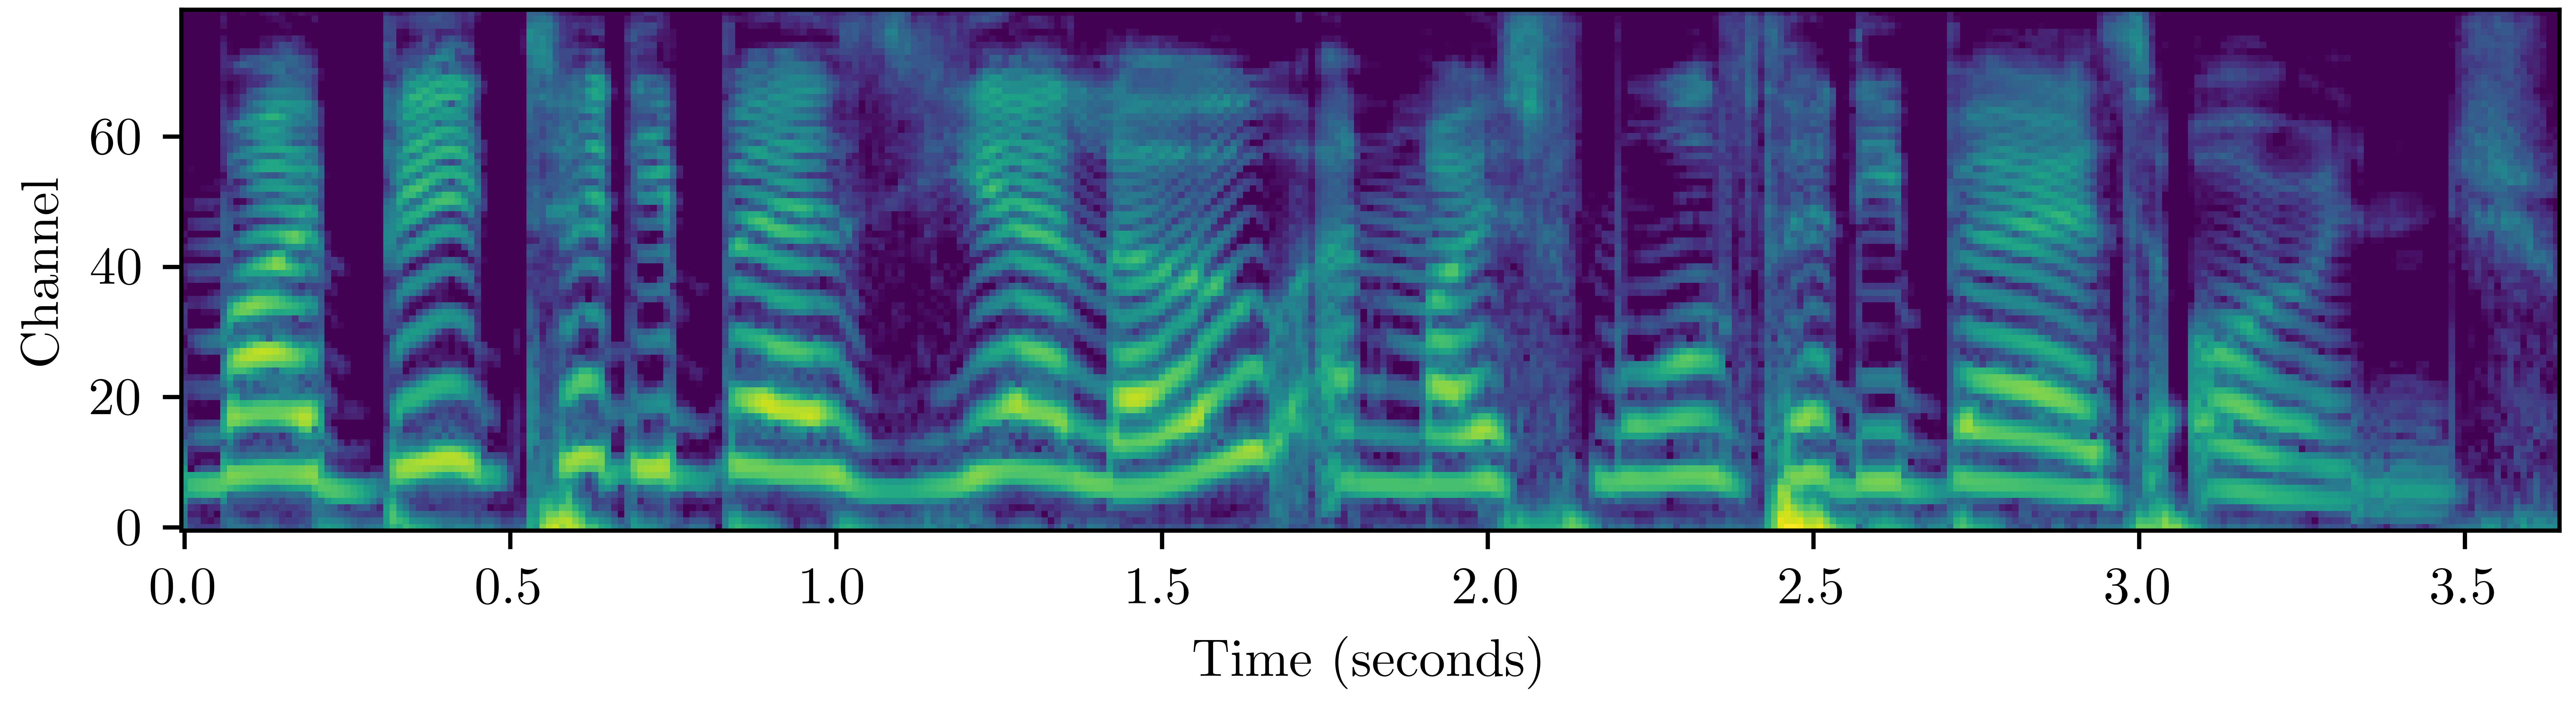
\includegraphics[width=\textwidth]{figures/specgram.png}
\centering 
\end{figure}

\mycomment{
        THIS IS WRONG / NEEDS CHANGING VVV
}
Whisper uses a natural language model to perform next-token prediction (in layperson's terms, there is a secondary system trying to ensure the intelligibility of sentences produced from transcription).
In a practical setting this means that conversational speech (i.e.\ speech which flows as sentences rather than semantically-disjoint terms) should be transcribed with a higher degree of accuracy.

Whisper is implemented in Python using the \emph{PyTorch}\cite{pytorch} library which allows computation to take place on GPUs which support CUDA, meaning transcripts can be generated very quickly on a high-performance computer (HPC) system.

\section{Confidence}
\mycomment{
       Write about what confidence is, then in subsections cover literature on the subject.
    }

\section{Speech Corpora}\label{sec:}
\mycomment{
  I think this section should be short and sweet. Just lay out what a corpus is, quick overview of the history of corpora, conversational corpora, 
}

\section{Transcription}\label{sec:transcription}
\mycomment{
    Perhaps move this down a bit?
  }

\subsection{Manual Transcription}\label{subsec:manual-transcription}

\subsection{Fully-Automatic Transcription}\label{subsec:full-auto-transcription}

\subsection{Semi-Automatic Transcription}\label{subsec:semi-auto-transcription}

\section{Summary}\label{sec:lit-survey-summary}
\mycomment{
    }
